\documentclass{article}

\usepackage{booktabs}
\usepackage{ctex}
\usepackage{float} % 用以支持 [H] 命令
\usepackage{amsmath}  % 导入 amsmath 包以支持数学命令
\usepackage{graphicx}  % 导入 graphicx 包以支持插图

\author{SwitZ \and Shichien \and Kylin-OIO}
\title{Write Anything Here}

\begin{document}

\maketitle

\section{Porter Robinson Discography}

\subsection{Worlds(2014)}

\begin{itemize}
    \item Divinity(feat. Amy Millan)
    \item Sad Machine
    \item Years of War(feat. Breanne Duren and Sean Caskey)
    \item Flicker
    \item Fresh Static Snow
    \item Hollowheart(2024)(feat. Amy Millan)
    \item Polygon Dust(feat. Lemaitre)
    \item Hear the Bells(feat. Imaginary Cities)
    \item Natural Light
    \item Lionhearted(feat. Urban Cone)
    \item Sea of Voices
    \item Fellow Feeling
    \item Goodbye to a World
    \item Shepherdess/She Heals Everything(2021)
\end{itemize}

\subsection{Nurture(2021)}

\begin{itemize}
    \item Lifelike
    \item Look at the Sky
    \item Get Your Wish
    \item Wind Tempos
    \item Musician
    \item Do-re-mi-fa-so-la-ti-do
    \item Mother
    \item Dullscythe
    \item Sweet Time
    \item Mirror
    \item Something Comforting
    \item Blossom
    \item Unfold(feat. Totally Enormous Extinct Dinosaurs)
    \item Trying to Feel Alive
    \item Fullmoon Lullaby(feat. Wednesday Campanella)
\end{itemize}

\subsection{SMILE!:D(2024)}

\begin{itemize}
    \item Knock Yourself Out XD
    \item Cheerleader
    \item Russian Roulette
    \item Perfect Pinterest Garden
    \item Year of the Cup
    \item Kistune Maison Freestyle
    \item Easier to Love You
    \item Mona Lisa
    \item Is There Really No Happiness?
    \item Everthing to Me
\end{itemize}

\section{冲突示例}

我是来捣蛋的。

\section{ Switz 的表格}

\begin{table}[H]
    \centering
    \begin{tabular}{lcr}
        \toprule
        \textbf{Column 1}                  & \textbf{Column 2}              & \textbf{Column 3}                   \\
        \midrule
        \textit{Left-aligned text}         & \textit{Centered text}         & \textit{Right-aligned text}         \\
        \texttt{Another left-aligned text} & \texttt{Another centered text} & \texttt{Another right-aligned text} \\
        \bottomrule
    \end{tabular}
    \caption{SwitZ 的表格}
    \label{tab:switz}
\end{table}

如表~\ref{tab:switz}所示,这是SwitZ的表格。
Hollowheart
如 \ref{tab:my_table} 所示,第三行第三列已改为代码字体。

\section{ Kylin-OIO 的表格}

\begin{table}[H]
    \centering
    \begin{tabular}{l c r}
        \toprule
        \textbf{Column 1}                  & \textbf{Column 2}              & \textbf{Column 3}                   \\
        \midrule
        \textit{Left aligned text}         & \textit{Centered text}         & \textit{Right aligned text}         \\
        \texttt{Another left aligned text} & \texttt{Another centered text} & \texttt{Another right aligned text} \\
        \bottomrule
    \end{tabular}
    \caption{三线表示例}
    \label{tab:my_table}
\end{table}

如 \ref{tab:my_table} 所示,第三行第三列已改为代码字体。

\section{数学代码}

行内公式使用一个美元符号包裹,如 $a^2 + b^2 = c^2$。

行间公式使用两个美元符号包裹,如

$$
    \int_{0}^{1} x^2 \, dx = \frac{1}{3}
$$

在数学公式中,使用下划线表示下标,使用脱字符表示上标,如 $a_{1}^{2}$。

如果只有一个字符作为上标或下标,可以省略大括号,如 $a^2$。

如果有多个字符要作为上标或者下标,需要大括号:$ \text{Deralive}_{\text{Kylin-OIO}}^{\text{Switz}} $

你会发现我把文本都用 \textbackslash text\{\} 包裹起来了,是因为在美元符号的公式环境中,不用包裹的文本会被解释为数学符号。

然后你会发现,Kylin-OIO 中间的这个横杠我进行了特殊处理,是因为有一些符号是不能随意打出来的,需要转义。
例如反斜杠、百分号(因为反斜杠是LateX 中的命令前缀,百分号是 LateX 中的注释,这些特殊的符号都需要转义。
转义的方法是在前面加上一个反斜杠,像我这样写 \%)

但是反斜杠的输入方法最特别,要使用一个命令来输出这个符号:\textbackslash

\LaTeX 的数学公式是有表格的,除了用 GPT 之外,还可以自己查表:

\begin{figure}[H]
    \centering
    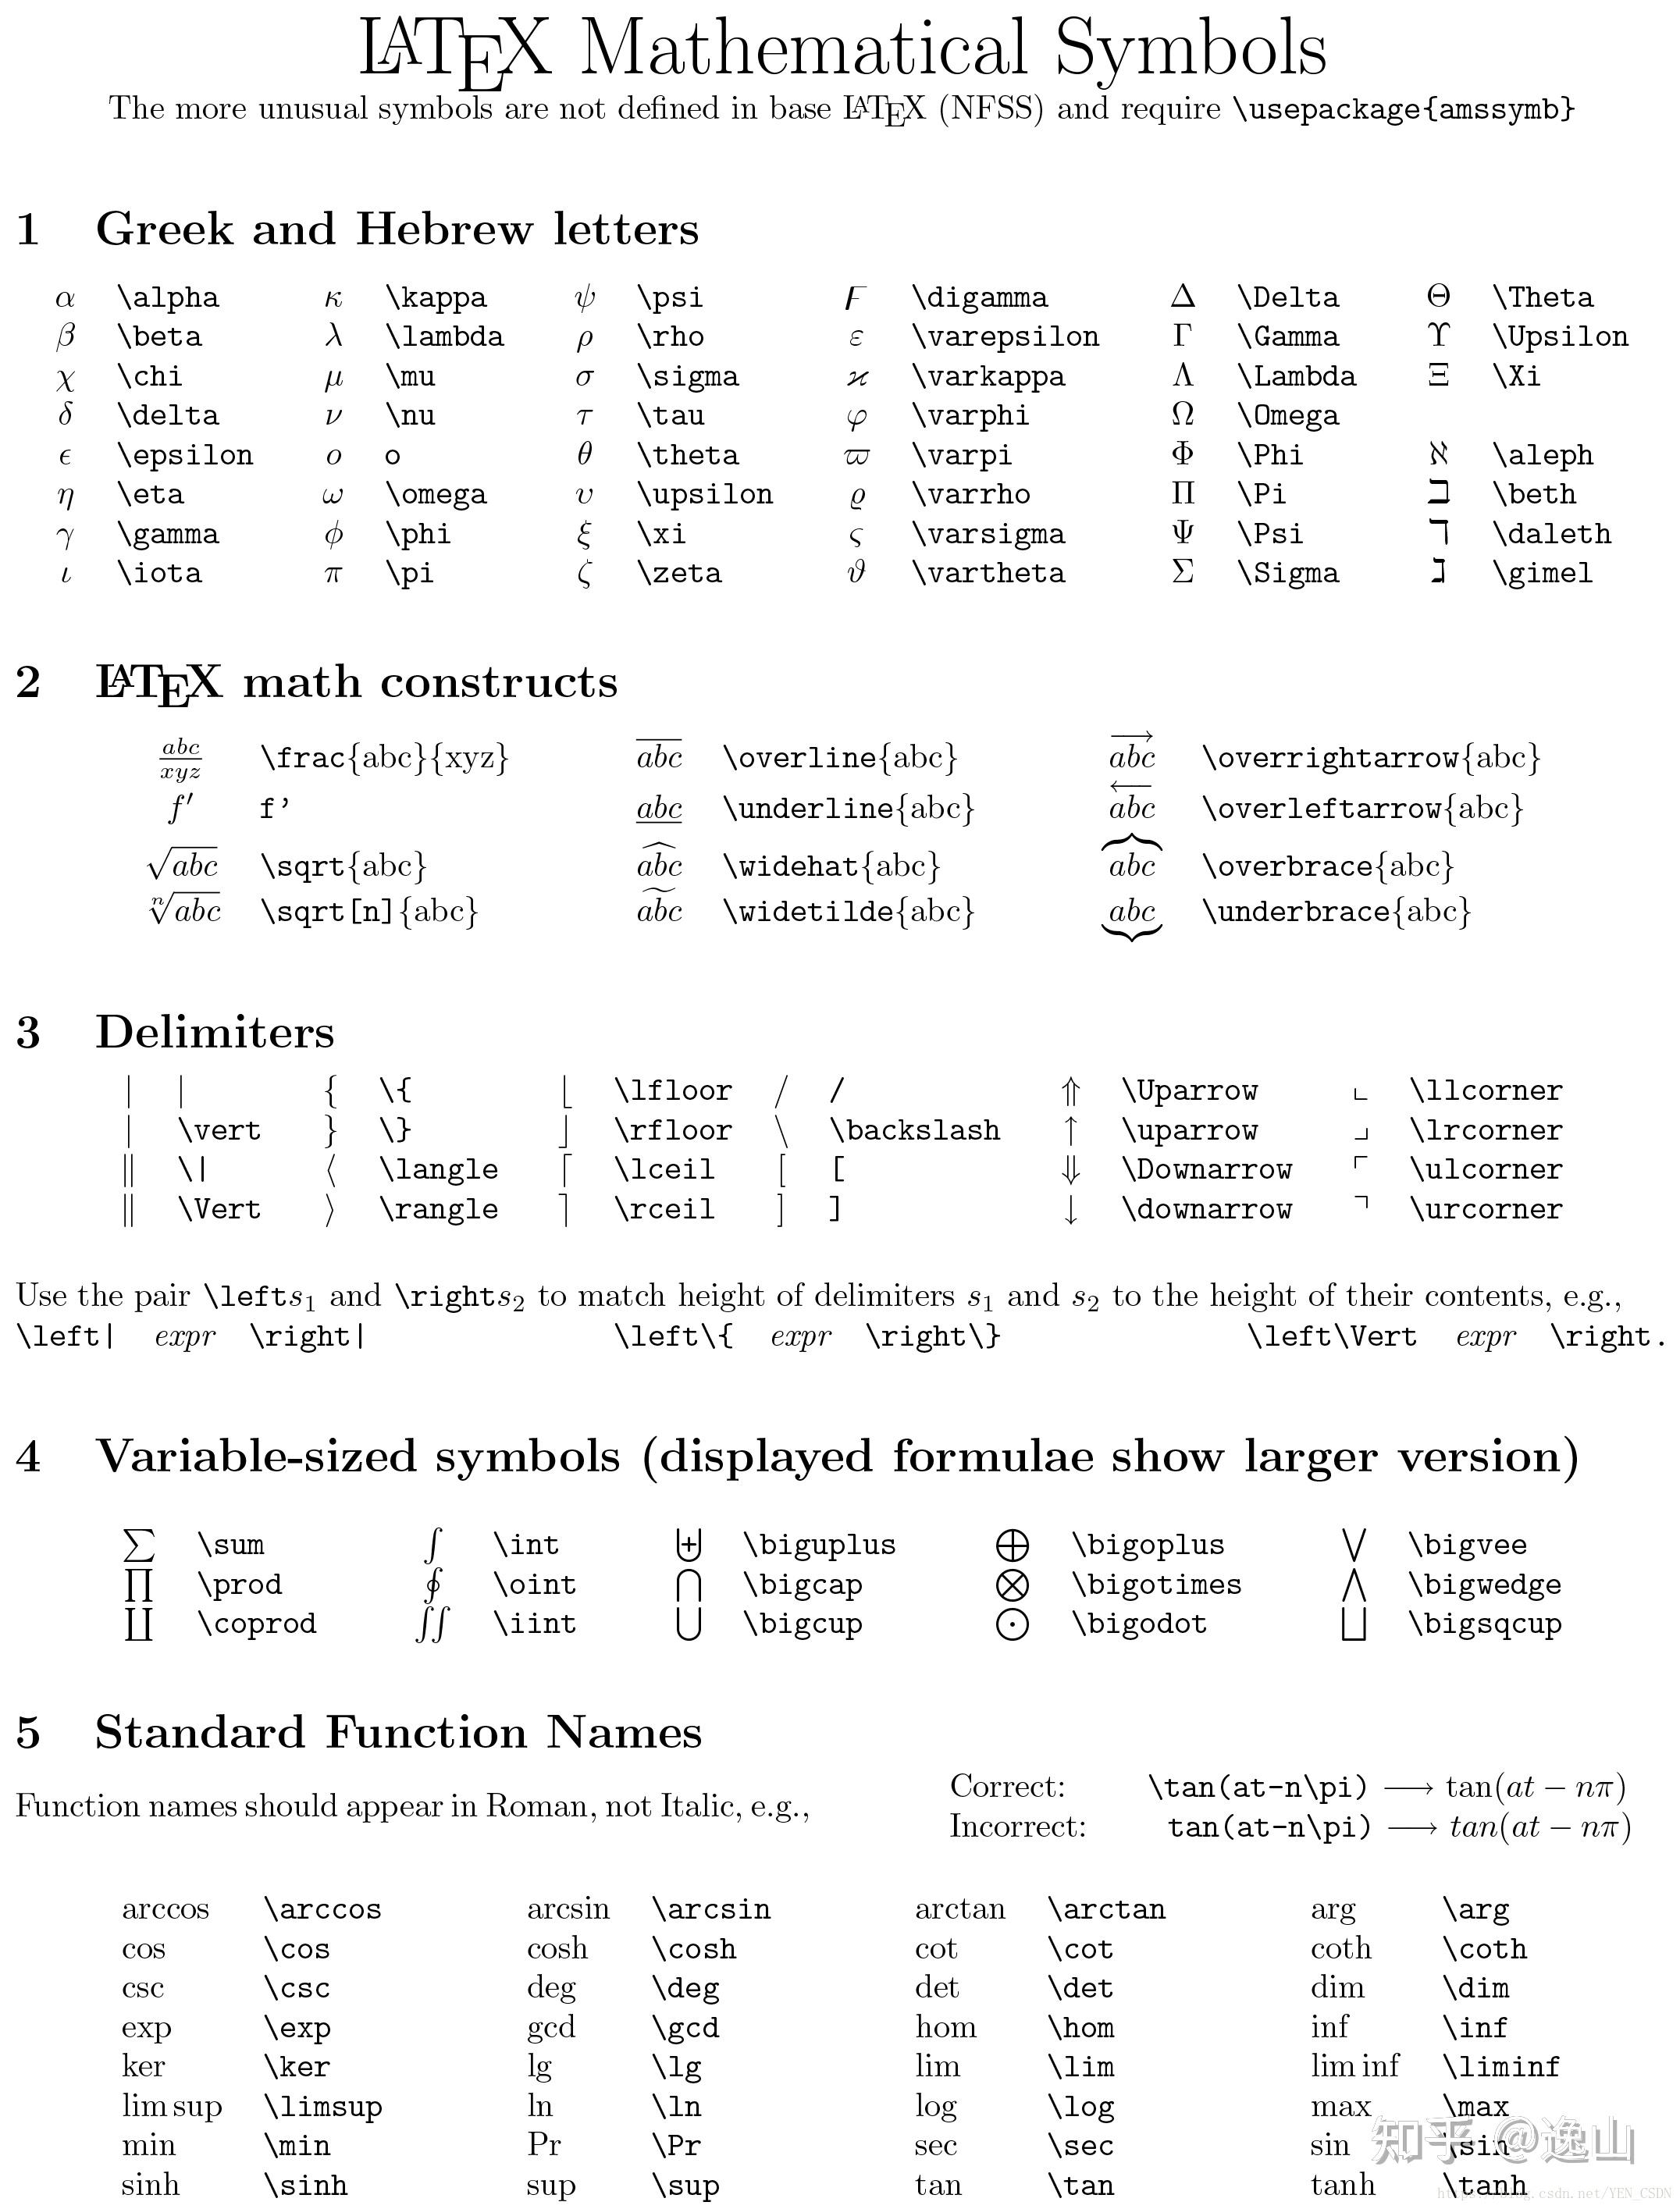
\includegraphics[width=0.99\textwidth]{img/latex-math-example.jpg}
    \caption{LateX 数学符号表}
    \label{fig:latex-math-symbols}
\end{figure}

\end{document}

